\documentclass[]{article}
\usepackage{lmodern}
\usepackage{amssymb,amsmath}
\usepackage{ifxetex,ifluatex}
\usepackage{fixltx2e} % provides \textsubscript
\ifnum 0\ifxetex 1\fi\ifluatex 1\fi=0 % if pdftex
  \usepackage[T1]{fontenc}
  \usepackage[utf8]{inputenc}
\else % if luatex or xelatex
  \ifxetex
    \usepackage{mathspec}
  \else
    \usepackage{fontspec}
  \fi
  \defaultfontfeatures{Ligatures=TeX,Scale=MatchLowercase}
\fi
% use upquote if available, for straight quotes in verbatim environments
\IfFileExists{upquote.sty}{\usepackage{upquote}}{}
% use microtype if available
\IfFileExists{microtype.sty}{%
\usepackage{microtype}
\UseMicrotypeSet[protrusion]{basicmath} % disable protrusion for tt fonts
}{}
\usepackage[margin=1in]{geometry}
\usepackage{hyperref}
\hypersetup{unicode=true,
            pdftitle={Домашнее задание №3},
            pdfauthor={datasalad},
            pdfborder={0 0 0},
            breaklinks=true}
\urlstyle{same}  % don't use monospace font for urls
\usepackage{color}
\usepackage{fancyvrb}
\newcommand{\VerbBar}{|}
\newcommand{\VERB}{\Verb[commandchars=\\\{\}]}
\DefineVerbatimEnvironment{Highlighting}{Verbatim}{commandchars=\\\{\}}
% Add ',fontsize=\small' for more characters per line
\usepackage{framed}
\definecolor{shadecolor}{RGB}{248,248,248}
\newenvironment{Shaded}{\begin{snugshade}}{\end{snugshade}}
\newcommand{\KeywordTok}[1]{\textcolor[rgb]{0.13,0.29,0.53}{\textbf{{#1}}}}
\newcommand{\DataTypeTok}[1]{\textcolor[rgb]{0.13,0.29,0.53}{{#1}}}
\newcommand{\DecValTok}[1]{\textcolor[rgb]{0.00,0.00,0.81}{{#1}}}
\newcommand{\BaseNTok}[1]{\textcolor[rgb]{0.00,0.00,0.81}{{#1}}}
\newcommand{\FloatTok}[1]{\textcolor[rgb]{0.00,0.00,0.81}{{#1}}}
\newcommand{\ConstantTok}[1]{\textcolor[rgb]{0.00,0.00,0.00}{{#1}}}
\newcommand{\CharTok}[1]{\textcolor[rgb]{0.31,0.60,0.02}{{#1}}}
\newcommand{\SpecialCharTok}[1]{\textcolor[rgb]{0.00,0.00,0.00}{{#1}}}
\newcommand{\StringTok}[1]{\textcolor[rgb]{0.31,0.60,0.02}{{#1}}}
\newcommand{\VerbatimStringTok}[1]{\textcolor[rgb]{0.31,0.60,0.02}{{#1}}}
\newcommand{\SpecialStringTok}[1]{\textcolor[rgb]{0.31,0.60,0.02}{{#1}}}
\newcommand{\ImportTok}[1]{{#1}}
\newcommand{\CommentTok}[1]{\textcolor[rgb]{0.56,0.35,0.01}{\textit{{#1}}}}
\newcommand{\DocumentationTok}[1]{\textcolor[rgb]{0.56,0.35,0.01}{\textbf{\textit{{#1}}}}}
\newcommand{\AnnotationTok}[1]{\textcolor[rgb]{0.56,0.35,0.01}{\textbf{\textit{{#1}}}}}
\newcommand{\CommentVarTok}[1]{\textcolor[rgb]{0.56,0.35,0.01}{\textbf{\textit{{#1}}}}}
\newcommand{\OtherTok}[1]{\textcolor[rgb]{0.56,0.35,0.01}{{#1}}}
\newcommand{\FunctionTok}[1]{\textcolor[rgb]{0.00,0.00,0.00}{{#1}}}
\newcommand{\VariableTok}[1]{\textcolor[rgb]{0.00,0.00,0.00}{{#1}}}
\newcommand{\ControlFlowTok}[1]{\textcolor[rgb]{0.13,0.29,0.53}{\textbf{{#1}}}}
\newcommand{\OperatorTok}[1]{\textcolor[rgb]{0.81,0.36,0.00}{\textbf{{#1}}}}
\newcommand{\BuiltInTok}[1]{{#1}}
\newcommand{\ExtensionTok}[1]{{#1}}
\newcommand{\PreprocessorTok}[1]{\textcolor[rgb]{0.56,0.35,0.01}{\textit{{#1}}}}
\newcommand{\AttributeTok}[1]{\textcolor[rgb]{0.77,0.63,0.00}{{#1}}}
\newcommand{\RegionMarkerTok}[1]{{#1}}
\newcommand{\InformationTok}[1]{\textcolor[rgb]{0.56,0.35,0.01}{\textbf{\textit{{#1}}}}}
\newcommand{\WarningTok}[1]{\textcolor[rgb]{0.56,0.35,0.01}{\textbf{\textit{{#1}}}}}
\newcommand{\AlertTok}[1]{\textcolor[rgb]{0.94,0.16,0.16}{{#1}}}
\newcommand{\ErrorTok}[1]{\textcolor[rgb]{0.64,0.00,0.00}{\textbf{{#1}}}}
\newcommand{\NormalTok}[1]{{#1}}
\usepackage{graphicx,grffile}
\makeatletter
\def\maxwidth{\ifdim\Gin@nat@width>\linewidth\linewidth\else\Gin@nat@width\fi}
\def\maxheight{\ifdim\Gin@nat@height>\textheight\textheight\else\Gin@nat@height\fi}
\makeatother
% Scale images if necessary, so that they will not overflow the page
% margins by default, and it is still possible to overwrite the defaults
% using explicit options in \includegraphics[width, height, ...]{}
\setkeys{Gin}{width=\maxwidth,height=\maxheight,keepaspectratio}
\IfFileExists{parskip.sty}{%
\usepackage{parskip}
}{% else
\setlength{\parindent}{0pt}
\setlength{\parskip}{6pt plus 2pt minus 1pt}
}
\setlength{\emergencystretch}{3em}  % prevent overfull lines
\providecommand{\tightlist}{%
  \setlength{\itemsep}{0pt}\setlength{\parskip}{0pt}}
\setcounter{secnumdepth}{0}
% Redefines (sub)paragraphs to behave more like sections
\ifx\paragraph\undefined\else
\let\oldparagraph\paragraph
\renewcommand{\paragraph}[1]{\oldparagraph{#1}\mbox{}}
\fi
\ifx\subparagraph\undefined\else
\let\oldsubparagraph\subparagraph
\renewcommand{\subparagraph}[1]{\oldsubparagraph{#1}\mbox{}}
\fi

%%% Use protect on footnotes to avoid problems with footnotes in titles
\let\rmarkdownfootnote\footnote%
\def\footnote{\protect\rmarkdownfootnote}

%%% Change title format to be more compact
\usepackage{titling}

% Create subtitle command for use in maketitle
\newcommand{\subtitle}[1]{
  \posttitle{
    \begin{center}\large#1\end{center}
    }
}

\setlength{\droptitle}{-2em}
  \title{Домашнее задание №3}
  \pretitle{\vspace{\droptitle}\centering\huge}
  \posttitle{\par}
  \author{datasalad}
  \preauthor{\centering\large\emph}
  \postauthor{\par}
  \predate{\centering\large\emph}
  \postdate{\par}
  \date{31/07/2017}

\usepackage[russian]{babel}

\begin{document}
\maketitle

Дано Х и Y (Х общий, а зависимая переменная у каждого подписана).
Необходимо построить диаграмму рассеяния (график Y от Х), гистограмму
распределения Y. Также нужно визуально оценить вид функциональной
зависимости и выбрать одну (можно и не одну) из предложенных моделей.
Для выбранной модели создать столбец расчитанных Y для заданных Х. Найти
разницу между заданным Y и расчитанным (ошибку модели), построить график
изменения ошибки от Х.

\subsection{Загрузка набора данных в R}\label{----r}

\begin{Shaded}
\begin{Highlighting}[]
\KeywordTok{setwd}\NormalTok{(}\StringTok{"~/Desktop/dz/visualization"}\NormalTok{)}
\NormalTok{dataset <-}\StringTok{ }\KeywordTok{read.csv}\NormalTok{(}\StringTok{"dz.csv"}\NormalTok{, }\DataTypeTok{header =} \OtherTok{TRUE}\NormalTok{, }\DataTypeTok{stringsAsFactors =} \OtherTok{FALSE}\NormalTok{)}

\KeywordTok{str}\NormalTok{(dataset)}
\end{Highlighting}
\end{Shaded}

\begin{verbatim}
## 'data.frame':    60 obs. of  2 variables:
##  $ X: num  0.1 0.2 0.3 0.4 0.5 0.6 0.7 0.8 0.9 1 ...
##  $ Y: num  -30.1 -38.2 -33.5 -27.8 -27.2 ...
\end{verbatim}

\begin{Shaded}
\begin{Highlighting}[]
\KeywordTok{summary}\NormalTok{(dataset)}
\end{Highlighting}
\end{Shaded}

\begin{verbatim}
##        X               Y          
##  Min.   :0.100   Min.   :-38.200  
##  1st Qu.:1.575   1st Qu.:-16.050  
##  Median :3.050   Median : -5.125  
##  Mean   :3.050   Mean   : -7.508  
##  3rd Qu.:4.525   3rd Qu.:  2.050  
##  Max.   :6.000   Max.   : 12.800
\end{verbatim}

\subsection{Диаграмма рассеяния (график Y от Х)}\label{---y--}

\begin{Shaded}
\begin{Highlighting}[]
\KeywordTok{library}\NormalTok{(ggplot2)}

\NormalTok{plot <-}\StringTok{ }\KeywordTok{ggplot}\NormalTok{(dataset, }\KeywordTok{aes}\NormalTok{(}\DataTypeTok{x =} \NormalTok{X, }\DataTypeTok{y =} \NormalTok{Y))}
\NormalTok{plot +}\StringTok{ }\KeywordTok{geom_point}\NormalTok{() +}\StringTok{ }\KeywordTok{ggtitle}\NormalTok{(}\StringTok{"XY scatterplot"}\NormalTok{)}
\end{Highlighting}
\end{Shaded}

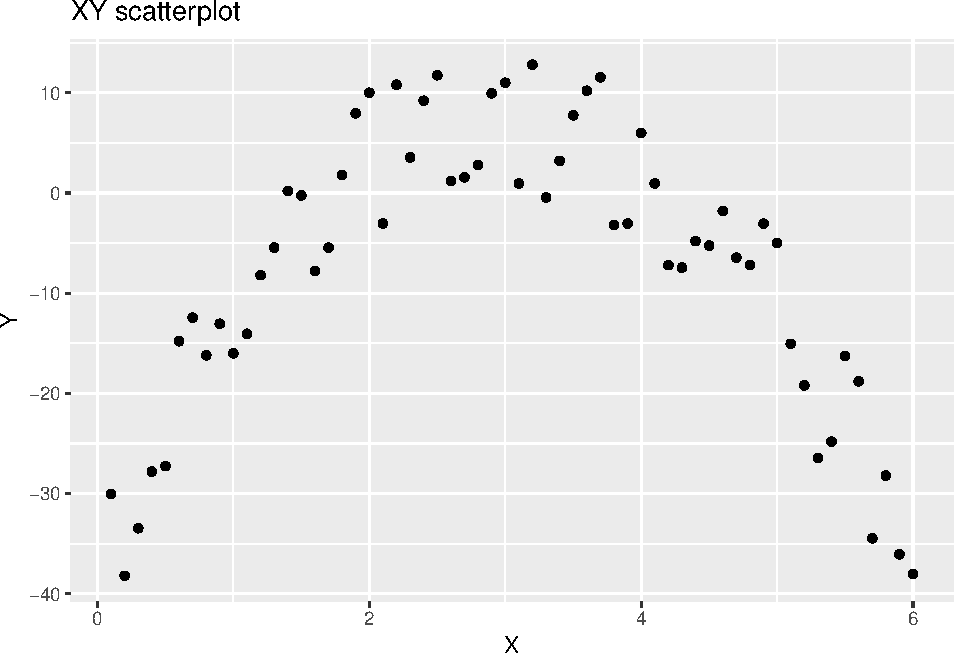
\includegraphics{DZ3_files/figure-latex/unnamed-chunk-2-1.pdf}

\subsection{Гистограмма распределения Y}\label{--y}

\begin{Shaded}
\begin{Highlighting}[]
\KeywordTok{qplot}\NormalTok{(Y, }\DataTypeTok{data =} \NormalTok{dataset, }\DataTypeTok{geom =} \StringTok{"histogram"}\NormalTok{, }\DataTypeTok{bins =} \DecValTok{100}\NormalTok{, }\DataTypeTok{main =} \StringTok{"Y histogram"}\NormalTok{)}
\end{Highlighting}
\end{Shaded}

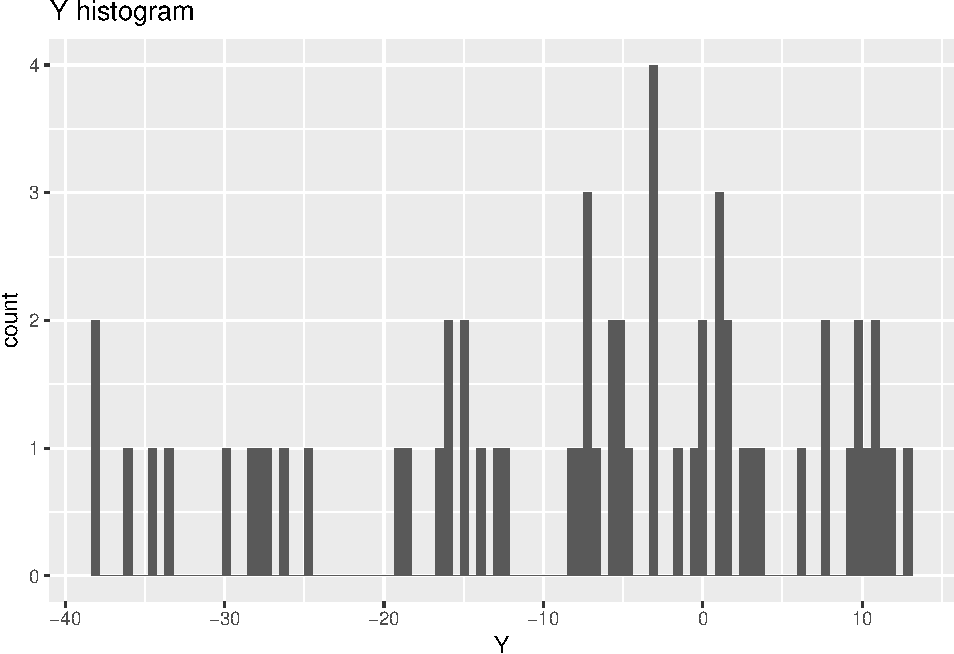
\includegraphics{DZ3_files/figure-latex/unnamed-chunk-3-1.pdf}

\subsection{Выбор модели}\label{-}

\begin{itemize}
\tightlist
\item
  y = 40,5*x-2,5
\item
  y = 0,5*x+10\\
\item
  y = 405,5*x-413
\item
  y = 10,11*x\^{}0,08\\
\item
  y = 103\emph{e\^{}(0,5}x)\\
\item
  y = -0,0015*x+0,0076\\
\item
  y = 0,01\emph{e\^{}(-0,5}x)\\
\item
  y = 58\emph{x\^{}2-206}x+262\\
\item
  y = -5\emph{x\^{}2+30}x-37
\end{itemize}

Расположение точек на диаграмме рассеивания напоминает параболу,
уходящую ветвями вниз, поэтому выберем последнюю модель: \textbf{y =
-5\emph{x\^{}2+30}x-37}

Для выбранной модели создаем столбец расчитанных Y для заданных Х.

\begin{Shaded}
\begin{Highlighting}[]
\NormalTok{f9 <-}\StringTok{ }\NormalTok{function(x) \{ -}\DecValTok{5} \NormalTok{*}\StringTok{ }\NormalTok{x^}\DecValTok{2} \NormalTok{+}\StringTok{ }\DecValTok{30} \NormalTok{*}\StringTok{ }\NormalTok{x -}\StringTok{ }\DecValTok{37} \NormalTok{\}}
\end{Highlighting}
\end{Shaded}

\begin{Shaded}
\begin{Highlighting}[]
\KeywordTok{library}\NormalTok{(dplyr)}

\NormalTok{data <-}\StringTok{ }\KeywordTok{tbl_df}\NormalTok{(dataset)}
\NormalTok{data <-}\StringTok{ }\KeywordTok{mutate}\NormalTok{(data, }\DataTypeTok{y9 =} \KeywordTok{f9}\NormalTok{(X))}
\end{Highlighting}
\end{Shaded}

\begin{Shaded}
\begin{Highlighting}[]
\KeywordTok{head}\NormalTok{(data)}
\end{Highlighting}
\end{Shaded}

\begin{verbatim}
## # A tibble: 6 x 3
##       X      Y     y9
##   <dbl>  <dbl>  <dbl>
## 1   0.1 -30.05 -34.05
## 2   0.2 -38.20 -31.20
## 3   0.3 -33.45 -28.45
## 4   0.4 -27.80 -25.80
## 5   0.5 -27.25 -23.25
## 6   0.6 -14.80 -20.80
\end{verbatim}

\begin{Shaded}
\begin{Highlighting}[]
\KeywordTok{summary}\NormalTok{(data)}
\end{Highlighting}
\end{Shaded}

\begin{verbatim}
##        X               Y                 y9         
##  Min.   :0.100   Min.   :-38.200   Min.   :-37.000  
##  1st Qu.:1.575   1st Qu.:-16.050   1st Qu.:-16.762  
##  Median :3.050   Median : -5.125   Median : -3.250  
##  Mean   :3.050   Mean   : -7.508   Mean   : -7.008  
##  3rd Qu.:4.525   3rd Qu.:  2.050   3rd Qu.:  4.987  
##  Max.   :6.000   Max.   : 12.800   Max.   :  8.000
\end{verbatim}

\begin{Shaded}
\begin{Highlighting}[]
\KeywordTok{qplot}\NormalTok{(}\DataTypeTok{x =} \NormalTok{X, }\DataTypeTok{y =} \NormalTok{Y, }\DataTypeTok{data =} \NormalTok{data)  +}\StringTok{ }\KeywordTok{geom_line}\NormalTok{(}\DataTypeTok{mapping =} \KeywordTok{aes}\NormalTok{(}\DataTypeTok{x =} \NormalTok{X, }\DataTypeTok{y =} \NormalTok{y9), }\DataTypeTok{col =} \StringTok{"red"}\NormalTok{) }
\end{Highlighting}
\end{Shaded}

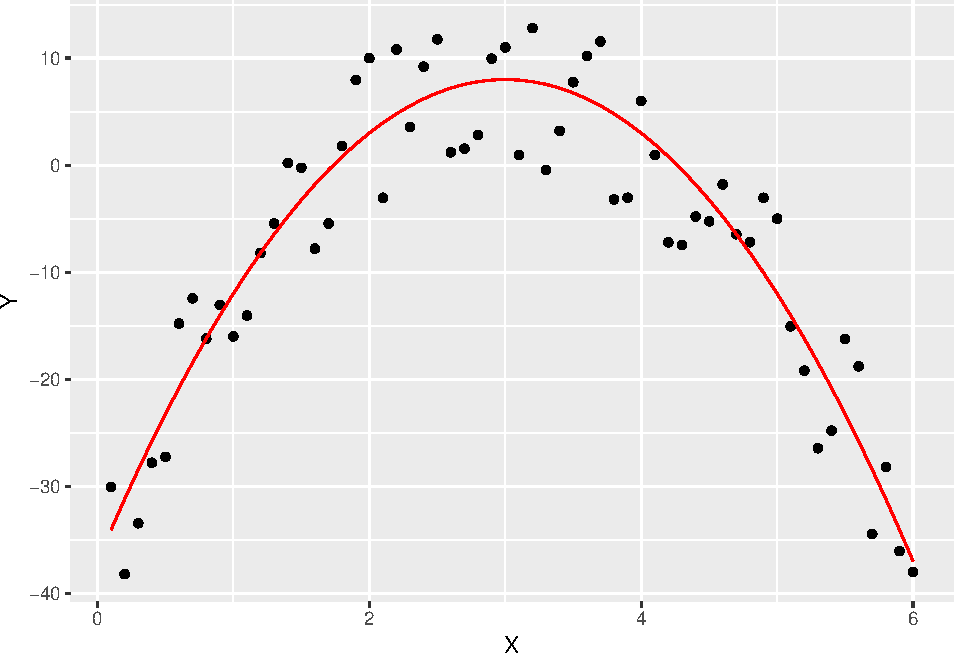
\includegraphics{DZ3_files/figure-latex/unnamed-chunk-6-1.pdf}

\subsection{Найти разницу между заданным Y и расчитанным (ошибку
модели), построить график изменения ошибки от
Х.}\label{----y----------.}

\begin{Shaded}
\begin{Highlighting}[]
\NormalTok{## Ошибка модели}
\NormalTok{data <-}\StringTok{ }\KeywordTok{mutate}\NormalTok{(data, }\DataTypeTok{diff =} \NormalTok{y9-Y)}
\KeywordTok{summary}\NormalTok{(data$diff)}
\end{Highlighting}
\end{Shaded}

\begin{verbatim}
##    Min. 1st Qu.  Median    Mean 3rd Qu.    Max. 
##   -7.00   -3.25    0.50    0.50    5.00    8.00
\end{verbatim}

\begin{Shaded}
\begin{Highlighting}[]
\NormalTok{## График изменения ошибки от Х}

\KeywordTok{qplot}\NormalTok{(X, diff, }\DataTypeTok{data =} \NormalTok{data, }\DataTypeTok{main =} \StringTok{"Model error by X"}\NormalTok{) +}\StringTok{ }\KeywordTok{geom_line}\NormalTok{()}
\end{Highlighting}
\end{Shaded}

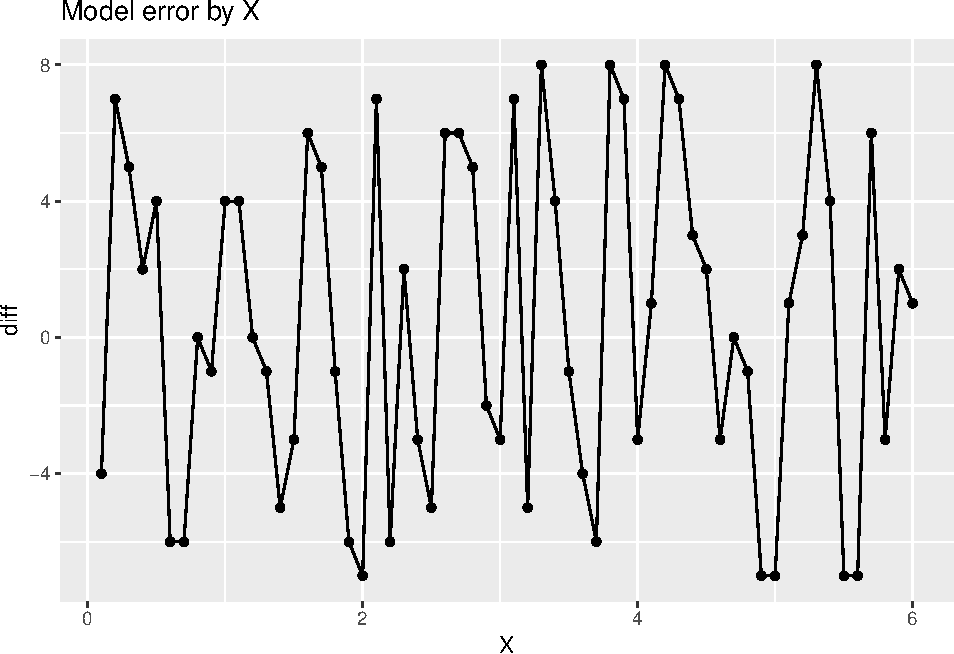
\includegraphics{DZ3_files/figure-latex/unnamed-chunk-8-1.pdf}


\end{document}
